
\documentclass[12pt,a4paper]{article}
\usepackage[UTF8]{ctex}
\usepackage{geometry}
\usepackage{graphicx}
\usepackage{booktabs}
\usepackage{longtable}
\usepackage{float}
\usepackage{xcolor}
\usepackage{fancyhdr}
\usepackage{hyperref}

% 頁面設定
\geometry{left=2.5cm,right=2.5cm,top=2.5cm,bottom=2.5cm}
\pagestyle{fancy}
\fancyhf{}
\fancyhead[L]{愛爾達綜合台劇集年齡分層收視分析報告}
\fancyhead[R]{\thepage}

% 標題設定
\title{\textbf{\Large 愛爾達綜合台劇集年齡分層收視分析報告}}
\author{資料分析團隊}
\date{2025年09月05日}

\begin{document}

\maketitle

\tableofcontents
\newpage

\section{執行摘要}

本報告基於愛爾達綜合台2024年全年ACNelson收視資料,進行深度年齡分層收視分析。
分析涵蓋8,981筆收視紀錄,
時間範圍為2024-01-01 至 2024-12-31,
包含143部劇集。

\subsection{主要發現}
\begin{itemize}
    \item 主要觀眾群:銀髮族(平均收視率 0.1140)
    \item 性別偏向:女性觀眾較多(差異 0.0219)
    \item 最佳收視時段:黃金時段(18-22點)
    \item 收視表現最佳月份:10月
    \item 收視表現最差月份:4月
\end{itemize}

\section{資料概況}

\begin{table}[H]
\centering
\caption{資料基本資訊}
\begin{tabular}{lr}
\toprule
項目 & 數值 \\
\midrule
總收視紀錄數 & 8,981 筆 \\
分析時間範圍 & 2024-01-01 至 2024-12-31 \\
涵蓋劇集數量 & 143 部 \\
分析生成日期 & 2025年09月05日 \\
\bottomrule
\end{tabular}
\end{table}

\section{年齡層收視偏好分析}

\subsection{整體年齡層收視率}

各年齡層的整體平均收視率如下表所示:

\begin{table}[H]
\centering
\caption{各年齡層整體平均收視率}
\begin{tabular}{lr}
\toprule
年齡群組 & 平均收視率 \\
\midrule
銀髮族 & 0.1140 \\
熟齡 & 0.0960 \\
青壯年 & 0.0914 \\
總體 & 0.0905 \\
核心觀眾 & 0.0804 \\
中年 & 0.0794 \\
年輕族群 & 0.0737 \\

\bottomrule
\end{tabular}
\end{table}

\subsection{主要劇集年齡偏好分析}

針對播出集數≥50集的主要劇集進行分析:

\begin{longtable}{lrrr}
\caption{主要劇集年齡偏好分析} \\
\toprule
劇集名稱 & 總集數 & 主要觀眾群 & 該群組收視率 \\
\midrule
\endfirsthead
\multicolumn{4}{c}{\textit{(續上表)}} \\
\toprule
劇集名稱 & 總集數 & 主要觀眾群 & 該群組收視率 \\
\midrule
\endhead
\bottomrule
\endfoot
蠟筆小新 & 2,332 & 熟齡 & 0.1092 \\
延禧攻略 & 308 & 銀髮族 & 0.2083 \\
後宮甄嬛傳 & 275 & 銀髮族 & 0.1345 \\
墨雨雲間 & 240 & 銀髮族 & 0.2218 \\
那年花開月正圓 & 217 & 銀髮族 & 0.0923 \\
琅琊榜 & 211 & 銀髮族 & 0.1416 \\
神鵰俠侶 & 176 & 銀髮族 & 0.1002 \\
月升滄海 & 170 & 銀髮族 & 0.1515 \\
醫師好辣 & 170 & 銀髮族 & 0.1053 \\
長相思 第一季 & 160 & 銀髮族 & 0.1649 \\

\end{longtable}

\section{時段收視分析}

不同時段的年齡層收視率分布:

\begin{table}[H]
\centering
\caption{各時段收視率分析}
\begin{tabular}{lrrrrrrr}
\toprule
時段 & 總體 & 核心觀眾 & 年輕族群 & 青壯年 & 中年 & 熟齡 & 銀髮族 \\
\midrule
凌晨時段 & 0.0137 & 0.0105 & 0.0096 & 0.0150 & 0.0095 & 0.0136 & 0.0149 \\
早晨時段 & 0.0525 & 0.0397 & 0.0308 & 0.0441 & 0.0475 & 0.0540 & 0.0737 \\
午間時段 & 0.1156 & 0.1036 & 0.0908 & 0.1180 & 0.1057 & 0.1154 & 0.1482 \\
黃金時段 & 0.1609 & 0.1503 & 0.1495 & 0.1677 & 0.1372 & 0.1807 & 0.1923 \\
深夜時段 & 0.0449 & 0.0439 & 0.0409 & 0.0596 & 0.0337 & 0.0520 & 0.0536 \\

\bottomrule
\end{tabular}
\end{table}

\section{性別收視差異分析}

\subsection{整體性別差異}

\begin{table}[H]
\centering
\caption{整體性別收視率比較}
\begin{tabular}{lr}
\toprule
性別 & 平均收視率 \\
\midrule
男性觀眾 & 0.0793 \\
女性觀眾 & 0.1012 \\
差異 & 0.0219 \\
偏向 & 女性觀眾 \\
\bottomrule
\end{tabular}
\end{table}

\subsection{各年齡層性別差異}

\begin{table}[H]
\centering
\caption{各年齡層性別差異分析}
\begin{tabular}{lrrrl}
\toprule
年齡層 & 男性 & 女性 & 差異 & 偏向 \\
\midrule
15-24歲 & 0.0698 & 0.0783 & 0.0085 & 女性 \\
25-34歲 & 0.0897 & 0.0933 & 0.0037 & 女性 \\
35-44歲 & 0.0772 & 0.0815 & 0.0044 & 女性 \\
45-54歲 & 0.0825 & 0.1075 & 0.0250 & 女性 \\
55歲以上 & 0.0910 & 0.1353 & 0.0443 & 女性 \\

\bottomrule
\end{tabular}
\end{table}

\section{月份收視趨勢分析}

\begin{table}[H]
\centering
\caption{各月份年齡層收視率}
\begin{tabular}{lrrrrrrr}
\toprule
月份 & 總體 & 核心觀眾 & 年輕族群 & 青壯年 & 中年 & 熟齡 & 銀髮族 \\
\midrule
1月 & 0.0826 & 0.0734 & 0.0708 & 0.0848 & 0.0676 & 0.0887 & 0.1067 \\
2月 & 0.0859 & 0.0757 & 0.0701 & 0.0870 & 0.0732 & 0.0928 & 0.1088 \\
3月 & 0.0957 & 0.0820 & 0.0727 & 0.0921 & 0.0844 & 0.1052 & 0.1239 \\
4月 & 0.0812 & 0.0682 & 0.0610 & 0.0771 & 0.0695 & 0.0845 & 0.1087 \\
5月 & 0.0857 & 0.0746 & 0.0743 & 0.0782 & 0.0747 & 0.0973 & 0.1090 \\
6月 & 0.0877 & 0.0774 & 0.0751 & 0.0816 & 0.0784 & 0.0966 & 0.1111 \\
7月 & 0.0938 & 0.0813 & 0.0771 & 0.0869 & 0.0835 & 0.1006 & 0.1170 \\
8月 & 0.0874 & 0.0745 & 0.0655 & 0.0837 & 0.0777 & 0.0907 & 0.1129 \\
9月 & 0.0928 & 0.0808 & 0.0686 & 0.0946 & 0.0835 & 0.0912 & 0.1223 \\
10月 & 0.1031 & 0.0968 & 0.0862 & 0.1166 & 0.0914 & 0.1052 & 0.1235 \\
11月 & 0.0982 & 0.0924 & 0.0822 & 0.1099 & 0.0884 & 0.1010 & 0.1163 \\
12月 & 0.0915 & 0.0866 & 0.0803 & 0.1024 & 0.0802 & 0.0964 & 0.1071 \\

\bottomrule
\end{tabular}
\end{table}

\subsection{各年齡層最佳/最差收視月份}

\begin{table}[H]
\centering
\caption{各年齡層最佳與最差收視月份}
\begin{tabular}{lrrrr}
\toprule
年齡群組 & 最佳月份 & 最佳收視率 & 最差月份 & 最差收視率 \\
\midrule
核心觀眾 & 10月 & 0.0968 & 4月 & 0.0682 \\
年輕族群 & 10月 & 0.0862 & 4月 & 0.0610 \\
青壯年 & 10月 & 0.1166 & 4月 & 0.0771 \\
中年 & 10月 & 0.0914 & 1月 & 0.0676 \\
熟齡 & 10月 & 0.1052 & 4月 & 0.0845 \\
銀髮族 & 3月 & 0.1239 & 1月 & 0.1067 \\
總體 & 10月 & 0.1031 & 4月 & 0.0812 \\

\bottomrule
\end{tabular}
\end{table}

\section{視覺化分析圖表}

\begin{figure}[H]
\centering
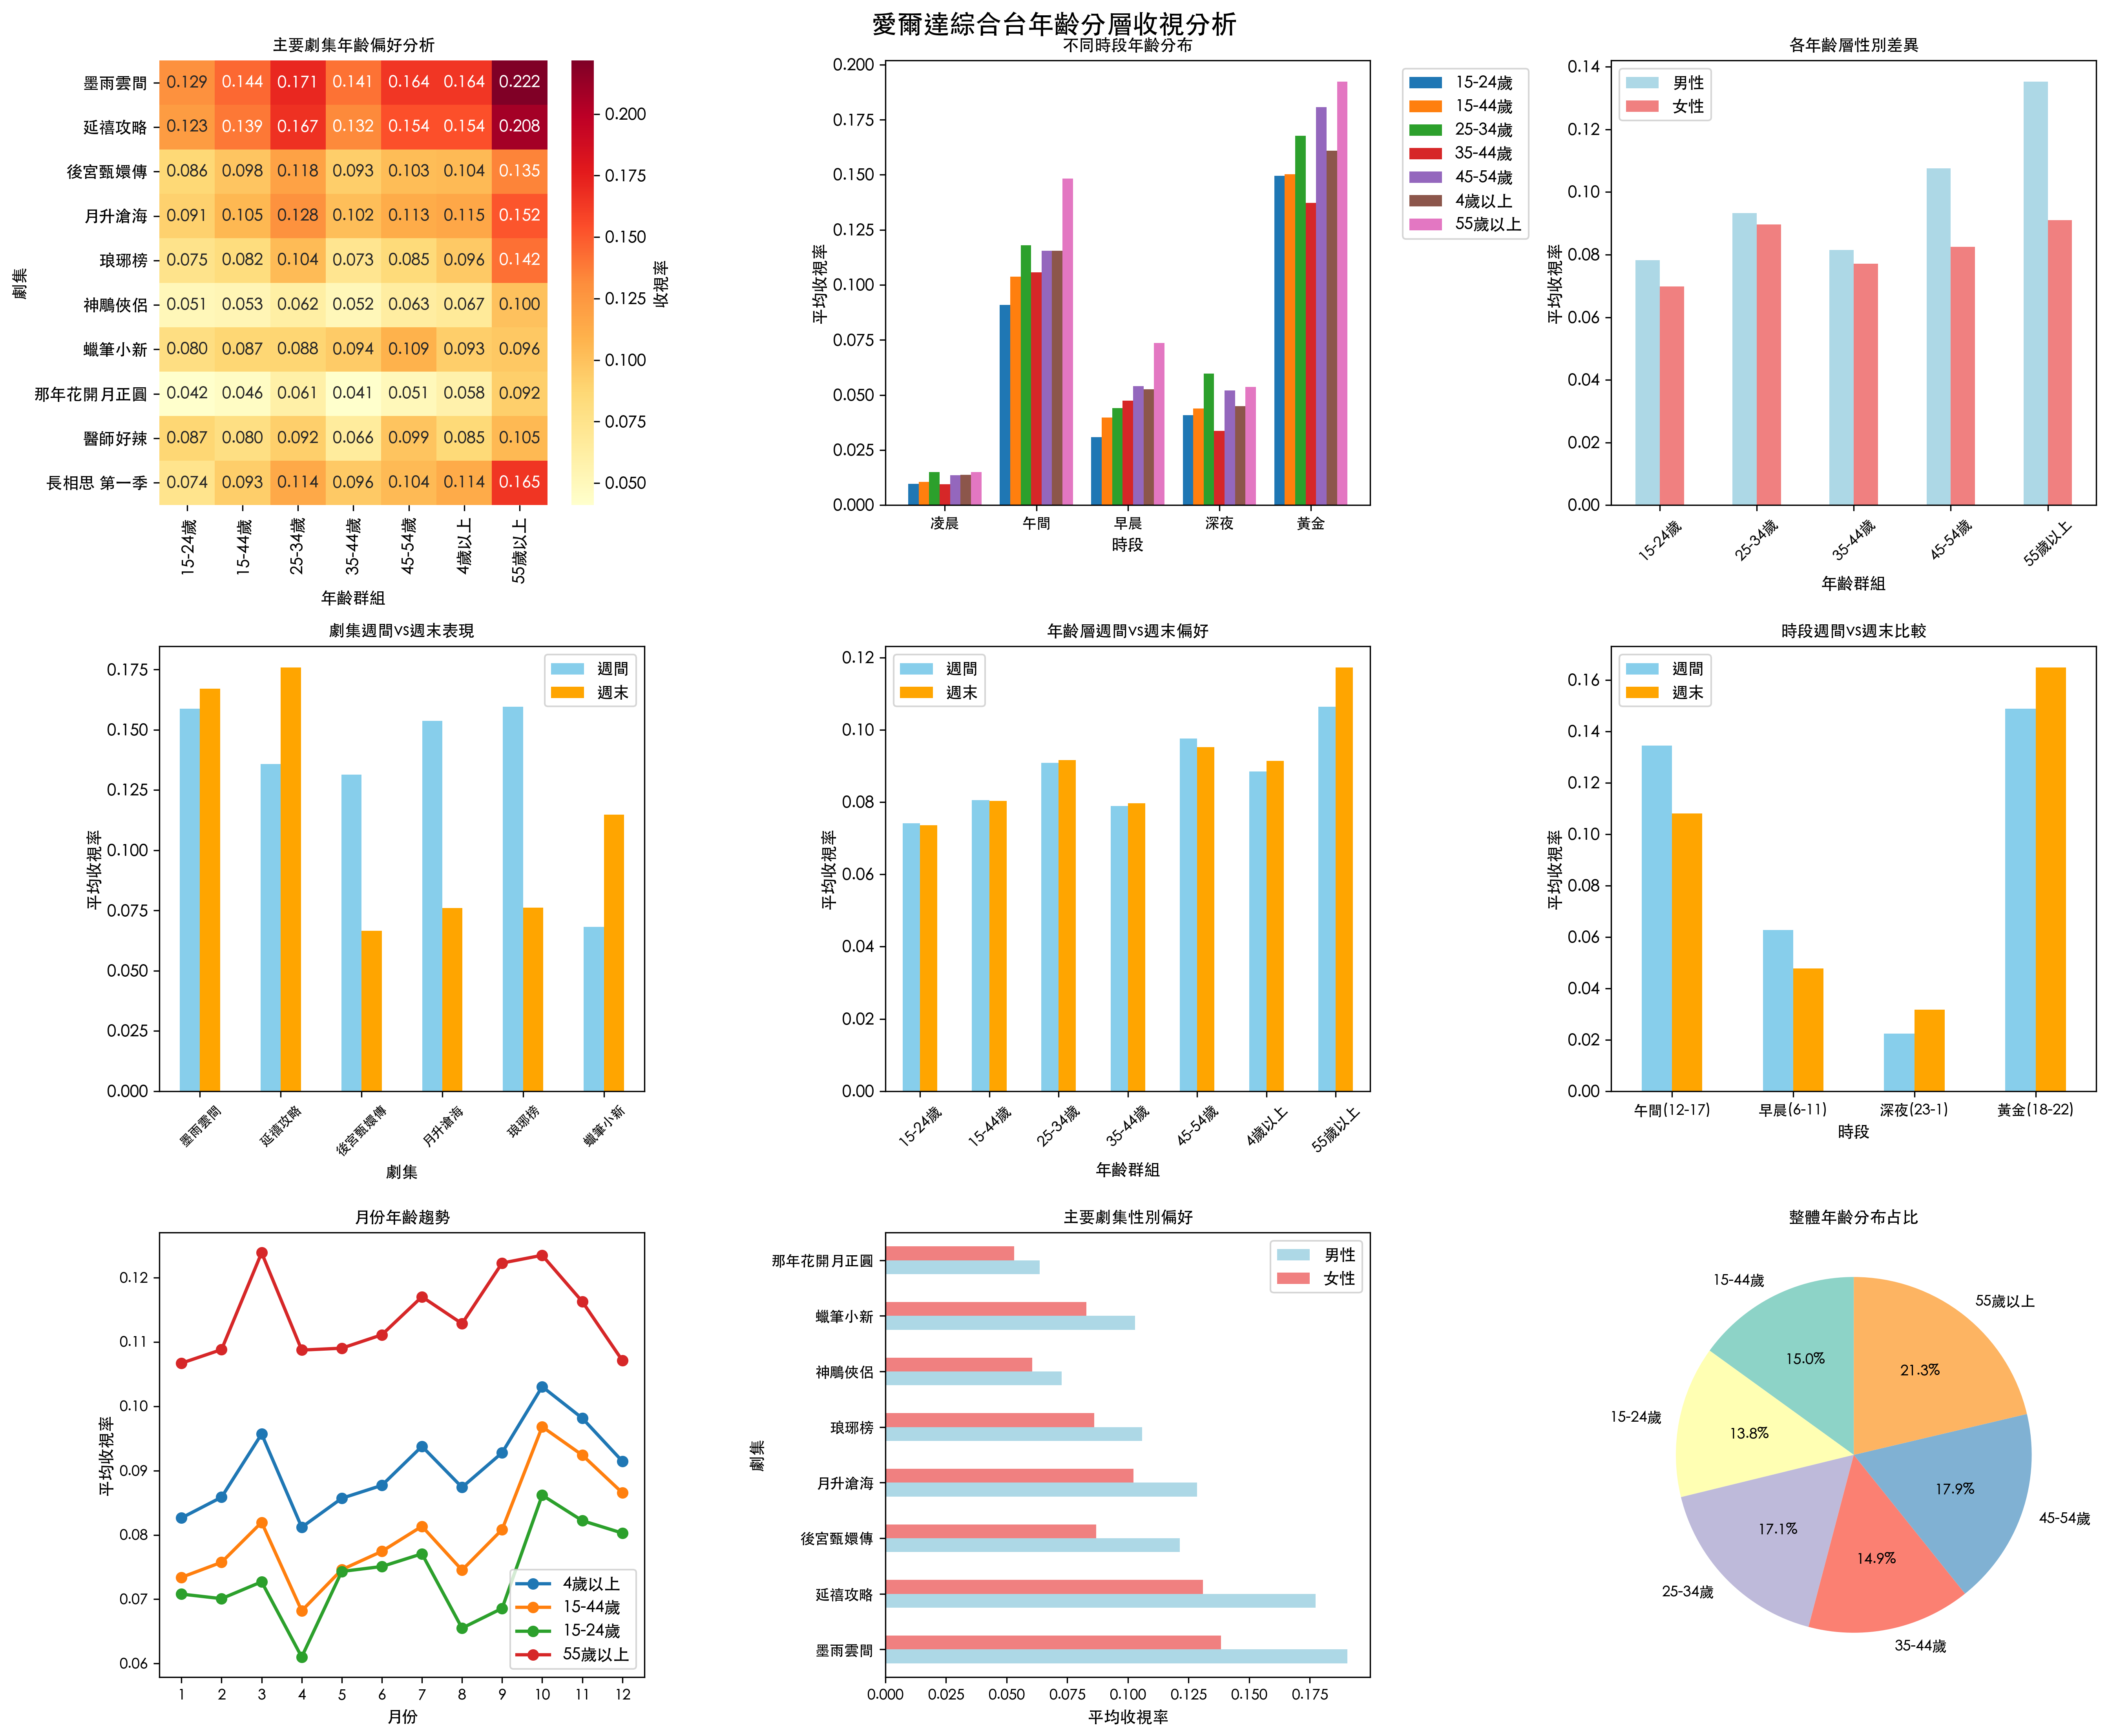
\includegraphics[width=\textwidth]{drama_age_analysis.png}
\caption{愛爾達綜合台年齡分層收視分析綜合圖表}
\label{fig:age_analysis}
\end{figure}

圖表包含六個分析面向:
\begin{enumerate}
    \item 主要劇集年齡偏好熱力圖
    \item 不同時段年齡分布
    \item 各年齡層性別差異
    \item 月份年齡趨勢
    \item 主要劇集性別偏好
    \item 整體年齡分布占比
\end{enumerate}

\section{策略建議}

基於以上分析結果,我們提出以下策略建議:

\subsection{觀眾定位策略}
\begin{itemize}
    \item 重點服務銀髮族和熟齡觀眾
    \item 針對女性觀眾偏好進行內容規劃
    \item 強化黃金時段節目品質
\end{itemize}

\subsection{節目編排建議}
\begin{itemize}
    \item 10月安排重點劇集首播
    \item 4月進行節目調整或重播安排
    \item 古裝劇和家庭劇較受銀髮族喜愛
\end{itemize}

\subsection{行銷策略}
\begin{itemize}
    \item 針對不同年齡層制定差異化行銷策略
    \item 重視女性觀眾的觀看偏好
    \item 善用黃金時段進行重要宣傳
\end{itemize}

\section{結論}

本分析報告基於2024年全年收視資料,深度剖析了愛爾達綜合台的年齡分層收視特徵。
主要發現銀髮族為最重要的觀眾群,女性觀眾整體收視偏好較高,
黃金時段為各年齡層的最佳收視時間。

建議電視台在未來的節目規劃中,重點關注銀髮族和熟齡觀眾的需求,
同時兼顧女性觀眾的觀看偏好,並善用黃金時段播出重點內容,
以提升整體收視表現。

\end{document}
